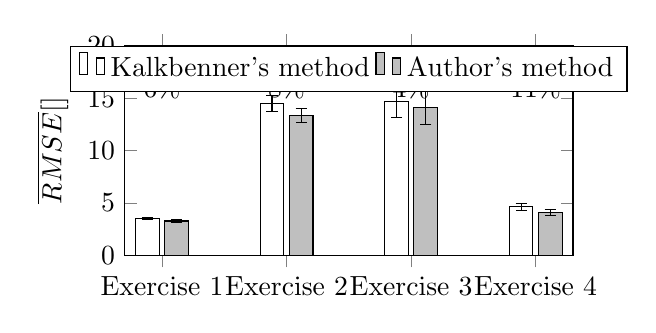
\begin{tikzpicture}
	\begin{axis}[
			ybar,
			bar width=.3cm,
			width=.6\textwidth,
			height=.35\textwidth,
			legend style={at={(0.5,1)},
				anchor=north,legend columns=-1},
			symbolic x coords={ex 1,ex 2,ex 3,ex 4},
			xtick=data,
			xticklabels={Exercise 1,Exercise 2,Exercise 3,Exercise 4},
			ymin=0,ymax=20,
			ylabel={$\overline{RMSE} [\degree]$},
		]
		\addplot [black,fill=white,error bars/.cd,y dir=both,y explicit] coordinates { 
			(ex 1,3.54) +- (0.0, 0.12)
			(ex 2,14.49) +- (0.0, 0.77)
			(ex 3,14.71) +- (0.0, 1.57)
			(ex 4,4.65)  +- (0.0, 0.32)
		};
		\addplot [black,fill=black!25,error bars/.cd,y dir=both,y explicit] coordinates { 
			(ex 1,3.29) +- (0.0, 0.12)
			(ex 2,13.35)+- (0.0, 0.65)
			(ex 3,14.08)+- (0.0, 1.55)
		(ex 4,4.11)  +- (0.0, 0.29)};
																																	
		\legend{Kalkbenner's method, Author's method}
		\node at (axis cs:ex 1,16){\textcolor{black}{6\%}};
		\node at (axis cs:ex 2,16){\textcolor{black}{8\%}};
		\node at (axis cs:ex 3,16){\textcolor{black}{4\%}};
		\node at (axis cs:ex 4,16){\textcolor{black}{11\%}};
	\end{axis}
\end{tikzpicture}	
	